\PassOptionsToPackage{unicode}{hyperref}
\PassOptionsToPackage{hyphens}{url}
\documentclass{article}
\setcounter{secnumdepth}{3}

\usepackage{amsmath,amssymb}
\usepackage{lmodern}
\usepackage{iftex}
\usepackage[letterpaper, margin=1in, top=1in, bottom=2in]{geometry}
\usepackage{listings}
\usepackage{color}
\usepackage{titling}
\usepackage{graphicx}
\usepackage{hyperref}
\usepackage[utf8]{inputenc}

\ifPDFTeX
  \usepackage[T1]{fontenc}
  \usepackage[utf8]{inputenc}
  \usepackage{textcomp} 
\else 
  \usepackage{unicode-math}
  \defaultfontfeatures{Scale=MatchLowercase}
  \defaultfontfeatures[\rmfamily]{Ligatures=TeX,Scale=1}
\fi
\IfFileExists{upquote.sty}{\usepackage{upquote}}{}
\IfFileExists{microtype.sty}{
  \usepackage[]{microtype}
  \UseMicrotypeSet[protrusion]{basicmath} 
}{}
\makeatletter
\@ifundefined{KOMAClassName}{
  \IfFileExists{parskip.sty}{
    \usepackage{parskip}
  }{
    \setlength{\parindent}{0pt}
    \setlength{\parskip}{6pt plus 2pt 2pt}}
}{
  \KOMAoptions{parskip=half}}
\makeatother
\usepackage{xcolor}
\usepackage{graphicx}

\makeatletter
\def\maxwidth{\ifdim\Gin@nat@width>\linewidth\linewidth\else\Gin@nat@width\fi}
\def\maxheight{\ifdim\Gin@nat@height>\textheight\textheight\else\Gin@nat@height\fi}
\makeatother
\setkeys{Gin}{width=\maxwidth,height=\maxheight,keepaspectratio}
\makeatletter
\def\fps@figure{htbp}
\makeatother
\setlength{\emergencystretch}{3em} 
\providecommand{\tightlist}{
  \setlength{\itemsep}{0pt}\setlength{\parskip}{0pt}}

\ifLuaTeX
  \usepackage{selnolig}  
\fi
\IfFileExists{bookmark.sty}{\usepackage{bookmark}}{\usepackage{hyperref}}
\IfFileExists{xurl.sty}{\usepackage{xurl}}{} 
\urlstyle{same}
\hypersetup{
  hidelinks,
  colorlinks=true,
  linkcolor=black,
  urlcolor=blue,
  pdfcreator={LaTeX via pandoc}}

\title{Game Engine Documentation}
\author{Coffee Time}
\date{}

\begin{document}

\maketitle
\includegraphics[width=\textwidth]{./assets/team_building.png}
\newpage

\tableofcontents
\newpage

\section{Profile}

\subsection{Introduction}
Game development requires programmers to either learn how to use a complex game engine or low level programming languages. Our solution aims to provide new game developers with a platform where they spend more time developing a game than managing graphics or I/O.

\subsection{Problem Description}
Game development requires the usage of low level programming languages or complicated game engines. There is a need for a high level programming language that can be used to develop games without having to manage input device peripherals or a graphical user interface.

\subsection{Objectives}

\subsubsection{General Objective}
Create a software solution, a platform that allows high level language programmers to develop games without worrying about a graphic user interface or I/O and instead spend more time developing the game.

\subsubsection{Specific Objectives}
\begin{itemize}
    \item Example games:
    \begin{itemize}
        \item A simple tic-tac-toe \href{https://docs.google.com/document/d/1MvlmgCBZvRrT61A3mnra-3bZ41zCcE_vmNHpHkZyQ2M/edit}{PRD Tictactoe}
        \item A generic Pac-Man \href{https://docs.google.com/document/d/1ST29Ap_2OGVEf--gPTfHYmAZrcIQC6jl6y32fM3UQWo/edit}{PRD Pacman}
    \end{itemize}
    \item Input peripherals support
    \begin{itemize}
        \item Keyboard
        \item Mouse
    \end{itemize}
    \item Output support
    \begin{itemize}
        \item Audio
        \item Graphical User Interface
    \end{itemize}
    \item Game Development Library
    \begin{itemize}
        \item This library will provide necessary tools for game development.
    \end{itemize}
\end{itemize}

\subsection{Scope and Limits}

\subsubsection{Scope}
\begin{itemize}
    \item Java developers that want to develop games.
\end{itemize}

\subsubsection{Limits}
\begin{itemize}
    \item Hardware
    \begin{itemize}
        \item A GPU that supports Vulkan, since version 1.3
    \end{itemize}
    \item Miscellany
    \begin{itemize}
        \item Games only can be played locally.
        \item Only 2D graphics.
        \item To run the game, the end-user has to have basic terminal knowledge.
        \item The library will be written in Java 17.
    \end{itemize}
\end{itemize}

\section{Theorical Framework}

\subsection{Technology justification}
Has a team we divided by front-end and back-end, front-end refered to games development and the library, for backend we manage screen and console, console has a interpreter and screen has the peace that contains GUI, input/output and sounds.

\subsubsection{Frontend}

The team agreed to use Java as a frontend language, taking into account that it is a high-level language, from an object-oriented paradigm that the team already knows and has worked with before.

\begin{tabular}{|l|c|c|}
\hline
Language & Must be an OOP language & Must provide a testing suite \\
\hline
Java & YES & JUnit 5 \\
\hline
C & NO & UNITY \\
\hline
\end{tabular}

\subsubsection{Backend}

\textbf{Rust}
\begin{itemize}
    \item Is a Low-Level and compiled language
    \item ``Rust is blazingly fast and memory-efficient: with no runtime or garbage collector, it can power performance-critical services, run on embedded devices, and easily integrate with other languages.'' – Rust-Performance
    \item Graphs management
    \begin{itemize}
        \item Window handling: 
        \begin{itemize}
            \item Wayland
            \item X11
        \end{itemize}
        \item Graphics
    \end{itemize}
    \item I/O access
    \begin{itemize}
        \item Rust provides a variety of libraries for operations like listening for keyboard or mouse events.
    \end{itemize}
    \item Foreign Function Interface Support
    \begin{itemize}
        \item \textbf{Java:}
        \begin{itemize}
            \item JNI Bindings for Rust is a library that allows us to:
            \begin{itemize}
                \item Implement native Java methods for JVM in Rust
                \item Call Java code from Rust
                \item Embed JVM in Rust applications and use any Java libraries
            \end{itemize}
    
        \end{itemize}
        \item \textbf{C:}
        \begin{itemize}
            \item For static linking, a build process must be performed for the C code based on a CMakeLists.txt configuration, where it uses the cmake dependency to create a library.
        
        \end{itemize}
    \end{itemize}
    \item Technology justification \href{https://docs.google.com/document/d/1OWdCxe9lFPcMpADiyAyRCWGAioo0fwIuzMuRER24MHM/edit}{Doc}
\end{itemize}
\subsection{Game Communication}
\subsubsection{Description}
\setlength{\parskip}{1em}
To observe o understand the flow of information, lets begin with the game.
The game is an implementation in Java that must define the attitudes, events that the game will have, the programming of when you win and when you lose, what happens if a character collides with something in its environment, etc..., it is the responsibility of the game. take care of everything related to the logic of the game and its actions such as creating its resources such as sounds or images, for which the game itself must implement those events, Obeying the contract.


The contract is a library implemented by the team, we are based on and take JavaFX as an example, a graphic library that in order to use it requires you to create certain components for its use, now we call this library within the team bridge since it works as a bridge between the game and console.


This communication works through JNI, which as we pointed out before would be the method used to communicate both languages based on the successful results of the spike referring to this implementation.


Once the information reaches the console, it will be processed by the intermediaries, the input/output intermediate, which will send the information through sockets to the screen.


Screen also has the sockets to guarantee communication with the console, it is also responsible for managing the RUST graphic library, which in this case we use "nannou" as a graphic library, in terms of GUI (sprites), Input (keyboard and mouse ), output (sounds).


For how it works lets think about a game in this case Pacman, we collide with a ghost, this event is handled by the game the "what will happen when it collides" the state of the game is updated, since Pacman is removed from the screen by who has lost a life, so Pacman's image must be updated on the screen, that information flows through the previously described flow to reach the screen as an update of Pacman's image based on his coordinates
\begin{itemize}
    \item More info on:  \href{https://tree.taiga.io/project/joseluis-teran-coffeetime/wiki/game-communication}{Game Communication}
      \item More info on:  \href{https://github.com/Pending-Name-21/arquitecture/blob/main/workspace.dsl}{Architecture} 
      \item More info on:  \href{https://github.com/Pending-Name-21/arquitecture/pull/12}{Actual Architecture PR} 
\end{itemize}

\hypertarget{methodology}{
\section{Methodology}\label{methodology}}

\hypertarget{roles}{
\subsection{ROLES}\label{roles}}

\hypertarget{roles-res}{
\subsubsection{Roles and Responsibilities}\label{roles-res}}

\hypertarget{teamlead}{
\paragraph{Team Lead}\label{teamlead}}
The Team Lead is responsible for overseeing the project, ensuring that all teams are working correctly for the project objectives, facilitates communication between teams, and address any issues that may arise.

\hypertarget{architec}{
\paragraph{Architect}\label{architec}}
The Architect is responsible for the design of the software solution for the project. He ensures that the architecture meets both the needs of the project. The Architect collaborates closely with the Development Teams to make sure that the implementation aligns with the architectural vision and standards.

\hypertarget{scrummaster}{
\paragraph{Scrum Master}\label{scrummaster}}
The Scrum Master facilitates the Agile process within the team. He organizes and conducts Scrum ceremonies such as Sprint Planning, Daily Stand-ups, Sprint Reviews, and Sprint Retrospectives.

\hypertarget{po}{
\paragraph{Product Owner}\label{po}}
The Product Owner is responsible for defining the product vision and managing the product backlog. He prioritizes tasks, ensuring that the team delivers features that provide the most value. The Product Owner communicates the project requirements and changes to the development teams.

\hypertarget{devteamrole}{
\paragraph{Development Team}\label{devteamrole}}

\textbf{\\Games Team}
The Games Team focuses on developing example games such as a tic-tac-toe and a Pac-Man. They work on implementing game logic. The Games Team collaborates closely with the Console Team to integrate input and output support.

\textbf{Console Team}
The Console Team is responsible for developing the support for input events like keyboard and mouse, as well as output support for audio and graphical user interfaces. They ensure that the platform can run the games.

\hypertarget{qateamrole}{
\paragraph{QA Team}\label{qateamrole}}
The QA Team ensures the quality of the software solution by conducting rigorous testing. They identify and report bugs. The QA Team works closely with the Development Teams to ensure that issues are resolved.

\hypertarget{devops}{
\paragraph{DevOps Infrastructure Team}\label{devops}}
The DevOps Infrastructure Team is responsible for setting up and maintaining the development and production environments. They manage the continuous integration and continuous deployment (CI/CD) pipelines.


\hypertarget{teamleadarchitect}{
\subsubsection{Team Lead \& Architect}\label{teamleadarchitect}}

\textbf{Team Lead:}
Fabian Romero Claros

\textbf{Architect:}
Gabriel Santiago Concha Saavedra

\begin{center}\rule{0.5\linewidth}{0.5pt}\end{center}

\hypertarget{sprint0}{
\subsubsection{Sprint 0}\label{sprint0}}

\textbf{Product Owner:}
Emanuel Galindo Corpa 

\textbf{Scrum Master: }
Jose Luis Terán Rocha

\hypertarget{qateam}{
\paragraph{QA Team}\label{qateam-0}}

\begin{itemize}
\tightlist
\item
  Ronaldo Miguel Ángel Mendoza Mallcu
\item
  Sebastián Barra Zurita
\item
  Jhael Arce Chavez
\end{itemize}

\hypertarget{devteam}{
\paragraph{Dev Team}\label{devteam-0}}

\begin{itemize}
\tightlist
\item
  Fabian Romero Claros
\item
  Gabriel Santiago Concha Saavedra
\item
  Josue Mauricio Prado Camacho
\item
  Luis Enrique Espinoza Vera
\item
  Luiggy Mamani Condori
\item
  Axel Javier Ayala Siles
\item
  Victor Leon Villca Silva
\item
  Alex Paca Meneses
\item
  Jose Luis Terán Rocha
\end{itemize}

\begin{center}\rule{0.5\linewidth}{0.5pt}\end{center}

\hypertarget{sprint1}{
\subsubsection{\texorpdfstring{\textbf{Sprint
1}}{Sprint 1}}\label{sprint1}}

\textbf{Product Owner: }
Alex Paca Meneses

\textbf{Scrum Master: }
Jose Luis Terán Rocha

\hypertarget{qateam-1}{
\paragraph{\texorpdfstring{\textbf{QA Team}}{QA Team}}\label{qateam-1}}

\begin{itemize}
\tightlist
\item
  Jhael Arce Chavez - \textbf{QA Lead}
\item
  Sebastian Barra Zurita
\item
  Ronaldo Miguel Angel Mendoza Mallcu
\end{itemize}

\hypertarget{devteam-1}{
\paragraph{\texorpdfstring{\textbf{Dev
Team}}{Dev Team}}\label{devteam-1}}

\paragraph{Front End Team}\label{front-end-team-1}

\begin{itemize}
\tightlist
\item
  Victor Leon Villca Silva ~- \textbf{Lead}
\item
  Emanuel Javier Galindo Corpa
\item
  Luis Enrique Espinoza Vera
\item
  Josue Mauricio Prado Camacho
\end{itemize}

\paragraph{Back End Team}\label{back-end-team-1}

\begin{itemize}
\tightlist
\item
  Alex Paca Meneses \textbf{- Lead}
\item
  Gabriel Santiago Concha Saavedra
\item
  Axel Javier Ayala Siles
\item
  Fabian Romero Claros
\item
  Luiggy Mamani Condori
\item
  Jose Luis Terán Rocha
\end{itemize}

\paragraph{DevOps / Infrastructure Team}\label{devops-team-1}

\begin{itemize}
\tightlist
\item
  Gabriel Santiago Concha Saavedra
\item
  Jose Luis Terán Rocha
\end{itemize}

\begin{center}\rule{0.5\linewidth}{0.5pt}\end{center}

\hypertarget{sprint2}{
\subsubsection{\texorpdfstring{\textbf{Sprint
2}}{Sprint 2}}\label{sprint2}}

\textbf{Product Owner: }
Alex Paca Meneses

\textbf{Scrum Master: }
Jose Luis Terán Rocha

\hypertarget{qateam-2}{
\paragraph{\texorpdfstring{\textbf{QA Team}}{QA Team}}\label{qateam-2}}

\begin{itemize}
\tightlist
\item
  Ronaldo Miguel Angel Mendoza Mallcu ~- \textbf{QA Lead}
\item
  Jhael Arce Chavez
\item
  Sebastian Barra Zurita
\end{itemize}

\hypertarget{devteam-2}{
\paragraph{\texorpdfstring{\textbf{Dev
Team}}{Dev Team}}\label{devteam-2}}

\paragraph{Front End Team}\label{front-end-team-2}

\begin{itemize}
\tightlist
\item
  Emanuel Javier Galindo Corpa - \textbf{Lead}
\item
  Victor Leon Villca Silva
\item
  Luis Enrique Espinoza Vera
\item
  Josue Mauricio Prado Camacho
\end{itemize}

\paragraph{Back End Team}\label{back-end-team-2}

\begin{itemize}
\tightlist
\item
  Axel Javier Ayala Siles - \textbf{Lead}
\item
  Gabriel Santiago Concha Saavedra
\item
  Alex Paca Meneses
\item
  Fabian Romero Claros
\item
  Luiggy Mamani Condori
\item
  Jose Luis Terán Rocha
\end{itemize}

\paragraph{DevOps / Infrastructure Team}\label{devops-team-2}

\begin{itemize}
\tightlist
\item
  Gabriel Santiago Concha Saavedra
\item
  Jose Luis Terán Rocha
\end{itemize}

\begin{center}\rule{0.5\linewidth}{0.5pt}\end{center}

\hypertarget{sprint3}{
\subsubsection{\texorpdfstring{\textbf{Sprint
3}}{Sprint 3}}\label{sprint3}}

\textbf{Product Owner:}
Alex Paca Meneses

\textbf{Scrum Master:}
Jose Luis Terán Rocha

\hypertarget{qateam-3}{
\paragraph{\texorpdfstring{\textbf{QA Team}}{QA Team}}\label{qateam-3}}

\begin{itemize}
\tightlist
\item
  Josue Mauricio Prado Camacho ~- \textbf{QA Lead}
\item
  Luis Enrique Espinoza Vera
\end{itemize}

\hypertarget{devteam-3}{
\paragraph{\texorpdfstring{\textbf{Dev
Team}}{Dev Team}}\label{devteam-3}}

\paragraph{Games Team}\label{games-team-3}

\begin{itemize}
\tightlist
\item
  Fabian Romero Claros ~-
  \textbf{Lead}
\item
  Ronaldo Miguel Angel Mendoza Mallcu
\item
  Jhael Arce Chavez
\item
  Victor Leon Villca Silva
\item
  Emanuel Galindo Corpa
\item
  Sebastian Barra Zurita
\end{itemize}

\paragraph{Console Team}\label{console-team-3}

\begin{itemize}
\tightlist
\item
  Luiggy Mamani Condori ~- \textbf{Lead}
\item
  Gabriel Santiago Concha Saavedra
\item
  Alex Paca Meneses
\item
  Axel Javier Ayala Siles
\item
  Jose Luis Terán Rocha
\end{itemize}

\paragraph{DevOps / Infrastructure Team}\label{devops-team-3}

\begin{itemize}
\tightlist
\item
  Gabriel Santiago Concha Saavedra
\item
  Jose Luis Terán Rocha
\end{itemize}

\begin{center}\rule{0.5\linewidth}{0.5pt}\end{center}

\hypertarget{sprint4}{
\subsubsection{\texorpdfstring{\textbf{Sprint
4}}{Sprint 4}}\label{sprint4}}

\textbf{Product Owner: }
Alex Paca Meneses

\textbf{Scrum Master: }
Ronaldo Miguel Angel Mendoza Mallcu

\hypertarget{devteam-4}{
\paragraph{\texorpdfstring{\textbf{Dev
Team}}{Dev Team}}\label{devteam-4}}

\paragraph{Games Team}\label{games-team-4}

\begin{itemize}
\tightlist
\item
  Fabian Romero Claros - \textbf{Lead}
\item
  Ronaldo Miguel Angel Mendoza Mallcu
\item
  Jhael Arce Chavez
\item
  Victor Leon Villca Silva
\item
  Emanuel Galindo Corpa
\item
  Sebastian Barra Zurita
\end{itemize}

\paragraph{Console Team}\label{console-team-4}

\begin{itemize}
\tightlist
\item
  Luiggy Mamani Condori - \textbf{Lead}
\item
  Gabriel Santiago Concha Saavedra
\item
  Alex Paca Meneses
\item
  Jose Luis Terán Rocha
\item
  Josue Mauricio Prado Camacho
\item
  Luis Enrique Espinoza Vera
\item
  Axel Javier Ayala Siles
\end{itemize}

\paragraph{DevOps / Infrastructure Team}\label{devops-team-4}

\begin{itemize}
\tightlist
\item
  Gabriel Santiago Concha Saavedra
\item
  Jose Luis Terán Rocha
\end{itemize}

\newpage

\hypertarget{ceremonies}{
\subsection{CEREMONIES}\label{ceremonies}}

\hypertarget{scrumofscrums}{
\subsubsection{Scrum of Scrums}\label{scrumofscrums}}

We will implement a Scrum of Scrums approach to facilitate coordination
among multiple teams. This will involve regular meetings among the team
leads to discuss progress, dependencies, and impediments that affect the
larger project.\\
We will work using the agile framework, so our ceremonies will be the
following:~

\hypertarget{dailyleadstandup}{
\subsubsection{Daily Lead Stand Up}\label{dailyleadstandup}}

To ensure coordination among team leads, we will have daily stand-up
meetings specifically for the leads of each sub-team, the team lead, the
PO and the architect.. These meetings will focus on high-level updates,
strategic decisions, and any cross-team dependencies or issues. The
meeting will be on Tuesdays and Thursdays after finishing the daily
stand ups of all the teams.

\hypertarget{sprintplanning}{
\subsubsection{Sprint Planning:}\label{sprintplanning}}

Every Monday will be our meetings where Dev and QA Team will follow the
next points:

\begin{itemize}
\tightlist
\item
  Use of \textbf{Poker Planning} to estimate the points of each US.

  \begin{itemize}
  \tightlist
  \item
    The story points will be defined by the complexity of development
    and QA team.
  \end{itemize}
\item
  While we are defining our \textbf{Sprint Goals} and prioritize of new
  US to work

  \begin{itemize}
  \tightlist
  \item
    During the meeting, we will clarify any ambiguities or doubts about
    the US, which can conduce to a refinement of the US that is
    considered as \textbf{Backlog Refinement} or \textbf{Backlog
    Grooming.}
  \end{itemize}
\end{itemize}

\hypertarget{sprintduration}{
\subsubsection{\texorpdfstring{\textbf{Sprint
Duration:}}{Sprint Duration:}}\label{sprintduration}}

\begin{itemize}
\tightlist
\item
  As a team, we define our sprint of 1 week.
\end{itemize}

\hypertarget{dailystandup}{
\subsubsection{Daily Stand Up:}\label{dailystandup}}

Daily stand-up meetings will be held by each sub-team to communicate
progress and discuss any roadblocks. The schedule for these daily
stand-ups will be set and agreed upon by each sub-team. The Scrum Master
must attend all daily stand-up meetings.

\begin{itemize}
\tightlist
\item
  Having the demo of the product and the report and metrics of QA Team
  during the Sprint.

  \begin{itemize}
  \tightlist
  \item
    In the final demo will present the entire product developed with
    some metrics about US and also, the whole metrics by QA Team.
  \end{itemize}
\end{itemize}

\hypertarget{sprintreview}{
\subsubsection{Sprint Review:}\label{sprintreview}}

Every Friday will take into account the following points:

\begin{itemize}
\tightlist
\item
  Review of the work that has been completed during the sprint.

  \begin{itemize}
  \tightlist
  \item
    What items have been completed?
  \item
    Do we some US for Carry Over?
  \end{itemize}
\item
  \textbf{Review of the Product Backlog:}

  \begin{itemize}
  \tightlist
  \item
    Current state of the product backlog, what items remains.
  \item
    Changes are made based on the feedback received by Dev and QA Team
    and any changes according PO needs.
  \end{itemize}
\item
  The team and PO will collaborate on what to work on next, helping to
  prioritize the next sprint's backlog.
\item
  We will review what US did not go well in the Sprint and how we will
  fix it.
\end{itemize}

\hypertarget{sprintretrospective}{
\subsubsection{Sprint Retrospective:}\label{sprintretrospective}}

Every Friday when finishing the Sprint, where we are gonna talk about
what went right, what went wrong and what can be improved for our next
iteration. Having feedback from the sprint review.

\begin{itemize}
\tightlist
\item
  While the meeting is happening, we will work on our \textbf{Action
  Items}.

  \begin{itemize}
  \tightlist
  \item
    Identifing things we should start doing, stop doing, and continue
    doing in future Sprints, as well as specific action items to
    implement these changes.
  \end{itemize}
\end{itemize}

\newpage

\hypertarget{artifacts}{
\subsection{ARTIFACTS}\label{artifacts}}

\hypertarget{productbacklog}{
\subsubsection{\texorpdfstring{\textbf{Product
Backlog}}{Product Backlog}}\label{productbacklog}}

We maintain a prioritized list of all the features, enhancements, bug
fixes, and other work needed to complete the project.
It\textquotesingle s our single source of truth for what needs to be
done.

\href{https://tree.taiga.io/project/joseluis-teran-coffeetime/backlog}{Link: Product Backlog in Taiga}.

\hypertarget{sprintbacklog}{
\subsubsection{\texorpdfstring{\textbf{Sprint
Backlog}}{Sprint Backlog}}\label{sprintbacklog}}

We select a subset of the Product Backlog items for a specific Sprint,
along with a plan for how to deliver them. It\textquotesingle s created
during the Sprint Planning meeting by the Development Team and serves as
a guide for our work during the Sprint.

\hypertarget{burndownchart}{
\subsubsection{\texorpdfstring{\textbf{Burn-Down
Chart}}{Burn-Down Chart}}\label{burndownchart}}

We use a representation of the amount of work remaining in the Sprint.
It shows our progress towards completing the Sprint\textquotesingle s
goal and helps us track whether we\textquotesingle re on track to finish
all planned work by the end of the Sprint.

\hypertarget{impedimentlog}{
\subsubsection{\texorpdfstring{\textbf{Impediment
Log}}{Impediment Log}}\label{impedimentlog}}

We keep a record of the impediments or problems of each team member per
day It\textquotesingle s used during our Daily Standup meeting to
~identify any issues that need to be addressed.

\href{https://jalafoundation.sharepoint.com/:f:/s/CoffeeTime/EvrueabkwZZPn-vQxfzknlcBg55BRdrfIEqUw9mxtrYNWg?e=JVZHfq}{Link: Impediment Logs Sheets}.


\hypertarget{startstopcontinueactionitems}{
\subsubsection{\texorpdfstring{\textbf{Start-Stop-Continue-Action
Items}}{Start-Stop-Continue-Action Items}}\label{startstopcontinueactionitems}}

We identify things we should start doing, stop doing, and continue doing
in future Sprints, as well as specific action items to implement these
changes. It helps us reflect on our process and make improvements for
future iterations.

\href{https://miro.com/app/board/uXjVKDO7l8M=/?share_link_id=7422815223}{Link: Start-Stop-Continue-Action Items in Miro}.

\newpage

\hypertarget{dordod}{
\subsection{DOR/DOD}\label{dordod}}

\hypertarget{definitionofready}{
\subsubsection{\texorpdfstring{\textbf{Definition of
Ready}}{Definition of Ready}}\label{definitionofready}}

\begin{itemize}
\tightlist
\item
  The story should have a clear description that indicates what it hopes
  to achieve and why it is important.
\item
  Clear criteria should be established indicating when the user story
  will be considered complete.
\item
  The necessary resources (such as people, tools) must be available to
  complete the story effectively.
\item
  Before a story can be considered ready for development, it must have
  been prioritized and estimated.
\end{itemize}

\hypertarget{definitionofdone}{
\subsubsection{\texorpdfstring{\textbf{Definition of
Done}}{Definition of Done}}\label{definitionofdone}}

\begin{itemize}
\tightlist
\item
  Code reviews must be performed by at least one and max two team
  members.
\item
  All issues identified during the code review should be fixed.
\item
  Unit Tests must be completed and successfully passed before a task is
  considered ready for delivery.
\item
  All methods and classes from the library must be documented.
\item
  The documentation in the library provided should be clear, concise, and adequately
  describe the functionality of the code.
\item
  The architecture defined by the team must be followed, including
  established design patterns and conventions.
\end{itemize}

\newpage

\hypertarget{workflow-gitflow}{
\subsection{WORKFLOW AND GITFLOW}\label{workflow-gitflow}}

\hypertarget{workflow}{
\subsubsection{Workflow:}\label{workflow}}

\hypertarget{availabilitysupporttime}{
\paragraph{Availability / Support
Time:}\label{availabilitysupporttime}}

\begin{itemize}
\tightlist
\item
  Monday - Wednesday - Friday: 14.30 - 16.30
\item
  Tuesday - Thursday: 14.30 - 17.30
\end{itemize}

\hypertarget{developer}{
\paragraph{Developer:}\label{developer}}

\begin{itemize}
\tightlist
\item
  \textbf{Identification of User Stories (US):} the team will be in
  charge of identifying the User Stories that must be developed. These
  are short, simple descriptions of a feature told from the end
  user\textquotesingle s perspective.
\item
  \textbf{Prioritization of User Stories:} based on several factors,
  such as the value they provide to the end user, the difficulty of
  implementation, the dependencies between them, etc.
\item
  \textbf{Assignment of User Stories:} assignment of each US to a member
  of the development team. This should be done taking into account the
  skills and abilities of each team member, as well as their current
  workload.
\item
  \textbf{Taiga Dashboard Update:} at each stage of development, we
  constantly update our Taiga dashboard to reflect progress.
\end{itemize}

\hypertarget{codereviewsnbsp}{
\paragraph{Code reviews:~}\label{codereviewsnbsp}}

\begin{itemize}
\tightlist
\item
  \textbf{Peer review:} when a developer finishes a task and uploads it
  to the repository (makes a commit), another developer or two developers on the team
  should review the code. Aiming to detect errors and improve code
  quality.
\item
  \textbf{Code review automation:} code review tools will be used to
  automate part of this process such as \textbf{CI/CD}. Helping detect
  code style issues, programming errors, and other code quality issues.
\end{itemize}

\hypertarget{readyforqa}{
\paragraph{Ready for QA:}\label{readyforqa}}

\begin{itemize}
\tightlist
\item
  Once a testeable US is finished, it goes to "Ready for QA" status, we notify the
\item
  In case issues are detected, we proceed to correct and it goes to "Ready for QA" again. If there are no problems, the US goes to production.
\end{itemize}

\hypertarget{qualitycontrolnbsp}{
\paragraph{Quality Control:~}\label{qualitycontrolnbsp}}

\begin{itemize}
\tightlist
\item
  We assign a US that can be tested to a member of the QA team.
\item
  In the QA phase, they will report the bugs found in the different US
  and will be notified in Taiga for further information on the section
  \textbf{Issues.}
\end{itemize}

\hypertarget{productionnbsp}{
\paragraph{Production:~}\label{productionnbsp}}

\begin{itemize}
\tightlist
\item
  After QA approval, we merge the US to production and continue to the
  next US.
\end{itemize}

\begin{center}\rule{0.5\linewidth}{0.5pt}\end{center}

\hypertarget{gitflow}{
\subsubsection{Gitflow}\label{gitflow}}

We want to separate the different modules into different repositories to
better control integration and continuous distribution (CI/CD)
independently.\\
The repositories will be independent from each other but will have a
logical relationship, so a Community will be created to add that
relationship.\\
There is a Git Workflow called Multi-Repo where this same approach is
used, although it will not take all the concepts such as the use of
macros, but we will retain the organization by logic and independent
development.~

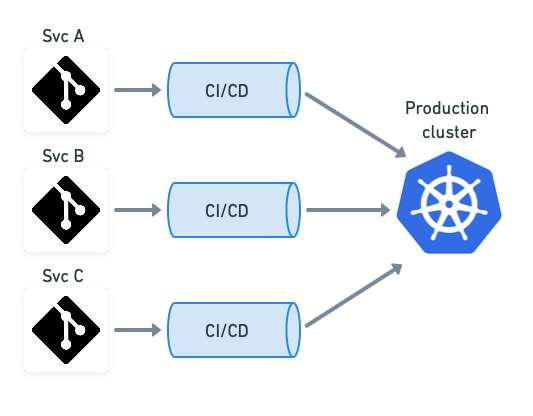
\includegraphics[width=\textwidth]{./methodology/src/assets/microdeployment.jpg}

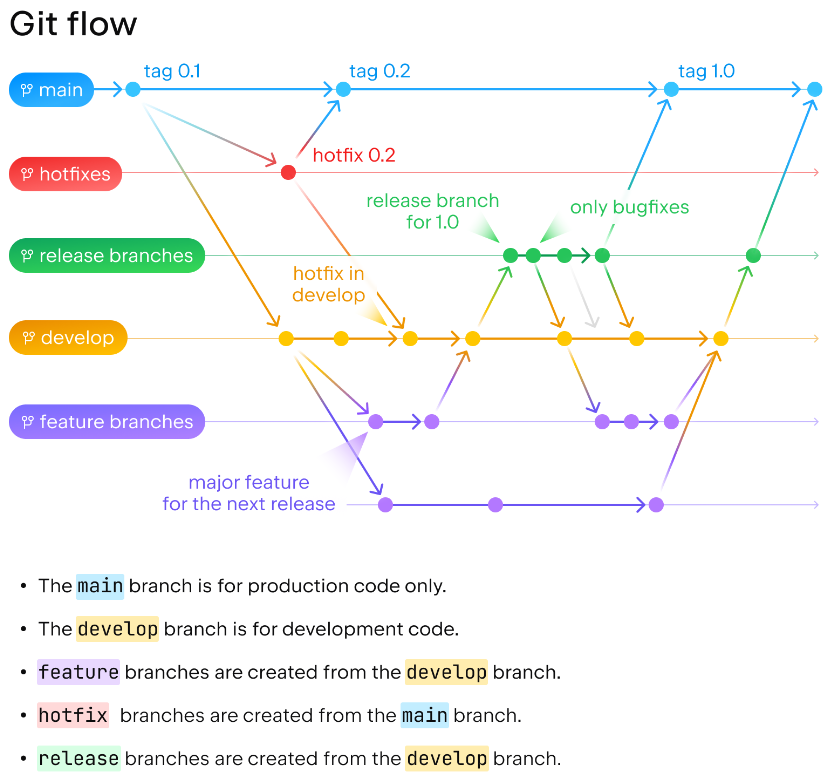
\includegraphics[width=\textwidth]{./methodology/src/assets/gitflow.png}

\hypertarget{conventionalcommits}{
\paragraph{Conventional Commits:}\label{conventionalcommits}}

\emph{A specification for adding human and machine readable meaning to
commit messages}

\begin{enumerate}
\tightlist
\item
  \textbf{fix:} fixes a bug or defect.
\item
  \textbf{feat:} adds a new feature or functionality.
\item
  \textbf{build}: changes related to the build system or dependencies.
\item
  \textbf{chore:} maintenance or housekeeping tasks.
\item
  \textbf{ci:} changes to continuous integration.
\item
  \textbf{docs:} documentation changes.
\item
  \textbf{style:} code appearance or formatting changes.
\item
  \textbf{refactor:} significant code restructuring without behavior
  change.
\item
  \textbf{perf:} performance improvements.
\item
  \textbf{test:} changes related to testing.
\end{enumerate}

\hypertarget{pullrequeststructurenbsp}{
\paragraph{Pull Request
structure:~}\label{pullrequeststructurenbsp}}

\begin{itemize}
\tightlist
\item
  \textbf{Pull Request Title:} Title should be clear and concise, and
  should accurately reflect the purpose of the change.
\item
  \textbf{Pull Request Description:} The description should provide
  details about what changes were made and why. You should include any
  relevant context that helps understand the change.

  \begin{itemize}
  \tightlist
  \item
    We will use the \textbf{Pull Request Template} and answer the
    following 3 questions:

    \begin{itemize}
    \tightlist
    \item
      What did I do?
    \item
      How did I do it?
    \item
      Why did I do it?
    \end{itemize}
  \end{itemize}
\item
  \textbf{References to Issues:} If the change is related to an issue in
  your issue tracking system (such as Jira, GitHub Issues, etc.), it
  should be mentioned in the description. This will help connect your
  pull request to the problem it is solving.
\item
  \textbf{Request Reviewers:} Ask one or more members of your team to
  review the pull request. They will provide feedback and suggest
  improvements if necessary.
\end{itemize}

\documentclass[a4paper,12pt]{article}
\usepackage[utf8]{inputenc}
\usepackage{amsmath}
\usepackage{amsfonts}
\usepackage{amssymb}
\usepackage{graphicx}
\usepackage{hyperref}

\title{Sprint Documentation}
\author{}
\date{}

\begin{document}

\maketitle

\tableofcontents
\newpage

\section{Sprint 0}
\subsection{Introduction}
In this sprint we were still researching concepts and tools, focused on low-level tools and languages for the console, also how to communicate console and game.
\subsection{Spikes}
We focus on the need to investigate and reduce uncertainty before committing to the implementation of concrete solutions.
\subsubsection{LLVM}
For LLVM, the research was concerned with finding a way to communicate a high-level language such as Java with a low-level language, at this point it was open to C, C++ or others, LLVM was an option that, although it fulfilled its ability to compile a high-level language to a low-level one, after doing the Spike we realized that it was more related to compilers, a set of tools to be able to make compilers even of industrial size, although we found something similar to what we were looking for with a tool developed with LLVM. "DragonEgg" But it is deprecated, the documentation is scarce and for the time of the project we did not see it optimal, it was discarded.
\subsubsection{JNI}
For JNI, which is Java Native Interface, a Spike was carried out to see its viability applied to a context close to the project, seeing what it could support and what not, to see its limitations, and this was the option that was taken for the project due to that the spike demonstrated effective communication between Java and Rust, so this concept was continued.
\subsection{POC's}
There POC on this Sprint its anexed on Product Backlog.
The results of the POC its the development of a technichal justification:
\begin{itemize}    
    \item Spike JVM: \href{https://docs.google.com/document/d/1OWdCxe9lFPcMpADiyAyRCWGAioo0fwIuzMuRER24MHM/edit#heading=h.ql4vc1ru9w5i}{Justification}
\end{itemize}


\subsection{Technical Justification}

During Sprint 0, the team focused exclusively on conducting Spikes instead of developing POCs (Proof of Concepts). This decision was made based on the following reasons:

\subsubsection{Reduction of Technical Uncertainty}
The project presented multiple areas of technical uncertainty that needed to be explored and understood before moving on to practical implementation. The Spikes allowed us to investigate different technologies, approaches, and possible solutions, providing a deeper understanding of the challenges and opportunities present.

\subsubsection{Feasibility Assessment}
Before committing significant resources to the development of POCs, it was crucial to assess the technical feasibility of the proposed ideas and approaches. The Spikes provided the opportunity to conduct brief and focused investigations, which allowed us to quickly identify viable solutions and discard those that were not, without the need to build complete implementations.


\subsection{High-Level Architecture (HLArchitecture)}
For the time of this Sprint there were no a first oficial version of the architecture, but the architecture that the SPikes and POC end of was the first version:
\begin{itemize}
\item Results: \href{https://github.com/Pending-Name-21/arquitecture/pull/1/files}{Architecture first version}
you can see it on: 
\item Link to C4 dsl: \href{https://structurizr.com/dsl}{Visualizer}
\end{itemize}
\newpage
\subsection{Product Backlog}

\subsubsection{Done}
Completed spikes.
\begin{itemize}
    \item Spike JVM: \href{https://tree.taiga.io/project/joseluis-teran-coffeetime/us/2?milestone=390348}{Task id-2}
    \item Spike C VM: \href{https://tree.taiga.io/project/joseluis-teran-coffeetime/us/4?milestone=390348}{Task id-4}
    \item Spike C++ VM: \href{https://tree.taiga.io/project/joseluis-teran-coffeetime/us/3?milestone=390348}{Task id-3}
    \item Spike Bytecode and C: \href{https://tree.taiga.io/project/joseluis-teran-coffeetime/us/5?milestone=390348}{Task id-5}
    \item Spike Reflection: \href{https://tree.taiga.io/project/joseluis-teran-coffeetime/us/6?milestone=390348}{Task id-6}
    \item Spike LLVM: \href{https://tree.taiga.io/project/joseluis-teran-coffeetime/us/8?milestone=390348}{Task id-8}
    \item Spike Sprites Sounds Effects: \href{https://tree.taiga.io/project/joseluis-teran-coffeetime/us/9?milestone=390348}{Task id-9}
    \item Spike Implicit calls in java: \href{https://tree.taiga.io/project/joseluis-teran-coffeetime/us/10?milestone=390348}{Task id-10}
    \item Spike KISS, DRYand YAGNI: \href{https://tree.taiga.io/project/joseluis-teran-coffeetime/us/12?milestone=390348}{Task id-12}
    \item Spike Assembler: \href{https://tree.taiga.io/project/joseluis-teran-coffeetime/us/13?milestone=390348}{Task id-13}
    \item Spike web Assamebly: \href{https://tree.taiga.io/project/joseluis-teran-coffeetime/us/14?milestone=390348}{Task id-14}
    \item Spike Interop communication between two programs: \href{https://tree.taiga.io/project/joseluis-teran-coffeetime/us/15?milestone=390348}{Task id-15}
    \item POC: Tech stack: \href{https://tree.taiga.io/project/joseluis-teran-coffeetime/us/16?milestone=390348}{Task id-16}
\end{itemize}

\subsubsection{Carry Over}
For this Sprint all assigned SPikes that were assigned ended in time. No carry overs.

\subsubsection{Conclussions}
This Sprite most work was on investigate ways to communicate a console in a low level language with the game, So all the Spikes were refered to understand a clair way to achieve that communication, all the spikes were ended on time, has a result of this spikes we choose JNI, has the way to communicate our game in Java with a console writed on Rust, also we discard LLVM, C VM, C++ VM and Assambly.
\end{document}


\section{Practical Framework}

\subsection{Sprint 3}

\subsubsection{Introduction}
During this sprint the team focused on the implementation of the input handler and input handler for bridge, as well as input management and sound management. The UMLs of each were assigned and based on these, implementation tasks were assigned based on the UMLs.

\subsubsection{POCs}

No proofs of concept (POCs) were conducted in this sprint.

\subsubsection{Technical Justification}
In Sprint 3 the decision was made to design the UMLs and implement them. The decision was made based on the following:

\begin{itemize}
    \item  Being able to handle keyboard and mouse events
    \item  Hear the sounds of the game through the console.
    \item  Communicate game with console.
    \item  Handle the updates of the information beetwen game and console.
\end{itemize}

\newpage

\subsubsection{Product Backlog}

\documentclass{article}
\setcounter{secnumdepth}{3}

\usepackage{amsmath,amssymb}
\usepackage{lmodern}
\usepackage{iftex}
\usepackage[letterpaper, margin=1in, top=0.5in, bottom=1in]{geometry}
\usepackage{listings}
\usepackage{color}
\usepackage{titling}
\usepackage{graphicx}
\usepackage{hyperref}
\usepackage{parskip}

\begin{document}

\maketitle

\hypertarget{burndownchart-s3}{
\section{Burn Down Chart}\label{Burn Down Chart S3}}
\href{https://tree.taiga.io/project/joseluis-teran-coffeetime/taskboard/sprint-3-8974}{Link: Sprint 3 Board on Taiga}.

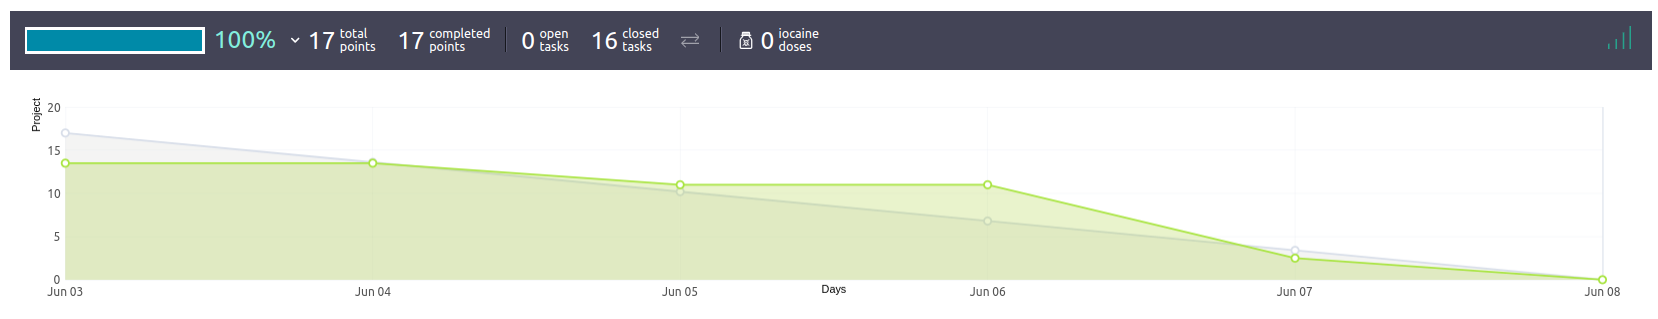
\includegraphics[width=\textwidth]{./assets/burndown-s3.png}

\hypertarget{startstopcontinueactionitems-s3}{
\section{Start-Stop-Continue-Action Items}\label{Start-Stop-Continue-Action Items S2}}
\href{https://miro.com/app/board/uXjVKDO7l8M=/?moveToWidget=3458764590247889881&cot=14}{Link: Start-Stop-Continue-Action Items Sprint 3 on Miro}.

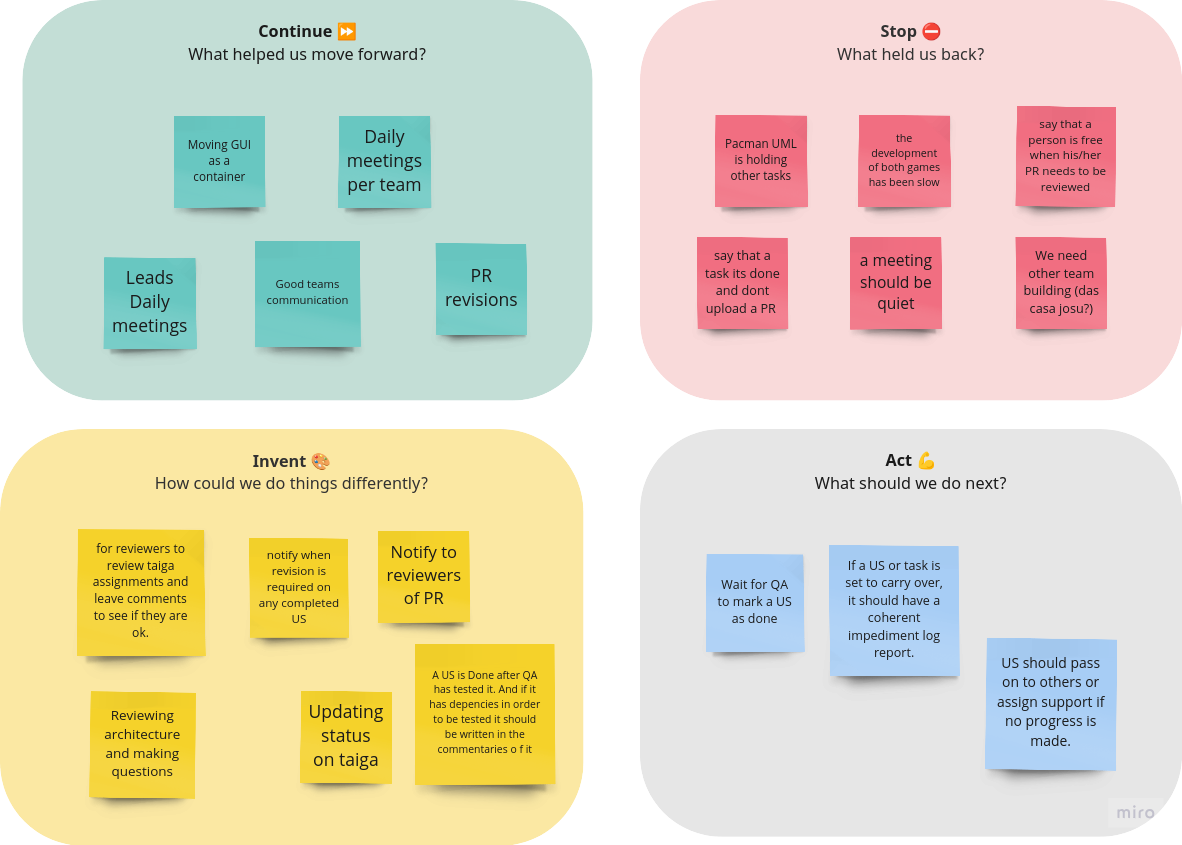
\includegraphics[width=\textwidth]{./assets/retrospective-s3.png}

\end{document}


\paragraph{Impediments}
For the impediments we registered on the following link:

\href{https://docs.google.com/spreadsheets/d/1hnMwOOVtyGWhViuAGwBsDpP79jTbHlJ09a_0gc9b4CM/edit?gid=1617748097#gid=1617748097}{impediments}

\paragraph{Conclusions}

For sprint 3 our goal was to implement in the project the different parts of the architecture to communicate with each other in the future, but this goal could not be fully achieved as some parts could not be implemented within the sprint duration.

\subsubsection{action items}

\begin{itemize}
    \item US should pass on to others or assign support if no progress is made.
    \item If a US or task is set to carry over, it should have a coherent impediment log report.
\end{itemize}

\subsubsection{Epics}

For Sprint 3 we have the following epics:

\begin{itemize}
    \item Input Management
    \item Sound management
    \item Input handler for the bridge
    \item Update Handler
    \item UML Pacman Game
    \item Render handler implementation 
\end{itemize}
\section{Practical Framework}
% \author{}
% \date{}

% \maketitle

\subsection{Sprint 1}

\subsubsection{Introduction}

In this sprint, our focus was on starting the contract for the developer and 
keep investigation about execution for the game using the console we define.
That's why we started with UMLs for our first game (Tic Tac Toe), console and
our contract (frontend-library), that is the Bridge.
At the same, we had been working on some Spikes for the console, such as to
define a graphic library for it, communication via JNI, apply shared memory 
between a game and console and finally, register input events, like mouse and keyboard.
All these Skipes were related in the context of the technologies used in the project.

\subsubsection{UMLs}

We had been starting on the UMLs for the contract, Tic Tac Toe game and console.

\begin{itemize}
    \item Task ID - 17: \href{https://tree.taiga.io/project/joseluis-teran-coffeetime/us/17?milestone=392128}{Console Diagram on Taiga (Comments Section)}
    \item Task ID - 18: \href{https://github.com/Pending-Name-21/arquitecture/pull/2}{Library UML Diagram on GitHub}
    \item Task ID - 22: \href{https://github.com/Pending-Name-21/arquitecture/pull/3}{Tic Tac Toe UML Diagram on GitHub}
\end{itemize}

\subsubsection{Spikes}

As we mentioned before, there were some Spikes to work with and here is the documentation generated by them:

\begin{itemize}    
    \item Task ID - 19: \href{https://docs.google.com/document/d/1a6wyQA0LM5thyAfOsWnkG-fTLcThvrsVPOGmFcoqkvw/edit?usp=sharing}{Graphic Libraries Documentation on Google Docs}
    \item Task ID - 20: \href{https://github.com/Pending-Name-21/console/tree/vm-spikes/jni_spike}{JNI Documentation on GitHub}
    \item Task ID - 21: \href{https://github.com/Pending-Name-21/console/blob/vm-spikes/shared-memory/README.md}{Shared Memory Documentation on GitHub}
    \item Task ID - 24: \href{https://universidadsalesian-my.sharepoint.com/:w:/g/personal/axel_ayala_9412013_usalesiana_edu_bo/EZlHobuXqW5AmffmDNnGaKYBdpordz1QlVJk88Pe_6S7HQ?e=DymfMq}{Input Listener Documentation on Word}
\end{itemize}

\subsubsection{POCs}

In this Sprint, we had no Proofs of Concept (POCs).

\subsubsection{Technical Justification}

During Sprint 1, the team exclusively focused on designing UMLs and
generating Spikes for console. This decision was based on the following reasons:

\subsubsection{High - Level Architecture}

The architecture followed in this sprint was based on the initial architecture.

\begin{itemize}
    \item Architecture: \href{https://github.com/Pending-Name-21/arquitecture/pull/1/files}{Architecture Initial Version}
    You can see it on: 
    \item C4 DSL: \href{https://structurizr.com/dsl}{Visualizer}
\end{itemize}

\newpage

\subsubsection{Epics}

For this Sprint 1, we have the following epics:

\begin{itemize}
    \item Bridge
    \item Console
    \item Graphics
    \item Games
\end{itemize}

\subsubsection{Sprint Backlog}

Completed Spikes and User Stories.

\begin{itemize}
    \item Task ID - 19: \href{https://tree.taiga.io/project/joseluis-teran-coffeetime/us/19?milestone=392128}{Spike Graphics Libraries for Console}
    \item Task ID - 20: \href{https://tree.taiga.io/project/joseluis-teran-coffeetime/us/20?milestone=392128}{Spike Console with JNI}
    \item Task ID - 21: \href{https://tree.taiga.io/project/joseluis-teran-coffeetime/us/21?milestone=392128}{Spike Shared Memory between Game - Console}
    \item Task ID - 24: \href{https://tree.taiga.io/project/joseluis-teran-coffeetime/us/24?milestone=392128}{Spike Mouse and Keyboard Events Listener}
    \item Task ID - 18: \href{https://tree.taiga.io/project/joseluis-teran-coffeetime/us/18?milestone=392128}{UML Library}
    \item Task ID - 22: \href{https://tree.taiga.io/project/joseluis-teran-coffeetime/us/22?milestone=392128}{UML Tic Tac Toe Game}
    \item Task ID - 17: \href{https://tree.taiga.io/project/joseluis-teran-coffeetime/us/17?milestone=392128}{UML Console}
    \item Task ID - 30: \href{https://tree.taiga.io/project/joseluis-teran-coffeetime/us/30?milestone=392128}{Frontend Library Implementation}
    \item Task ID - 35: \href{https://tree.taiga.io/project/joseluis-teran-coffeetime/us/35?milestone=392128}{Tic Tac Toe Mockups and Sprites}    
\end{itemize}

\subsubsection{Conclusions}

In Sprint 1, our focus was give that initial step in the game and the console, 
also of reviewing some documentation for our spikes. The most important goals
achieved were complete the UML for the contract and console too, besides of 
defining the graphic library, working with JNI, register input events and apply 
shared memory between the game and console.

\section{Practical Framework}
% \author{}
% \date{}

% \maketitle

\subsection{Sprint 2}

\subsubsection{Introduction}



\subsubsection{UMLs}



\begin{itemize}
    \item Task ID - 72: \href{https://github.com/Pending-Name-21/arquitecture/pull/11}{Pacman UML Diagram on GitHub}
\end{itemize}

\subsubsection{Spikes}

There were no Spikes

\subsubsection{POCs}

In this Sprint, we had no Proofs of Concept (POCs).

\subsubsection{Technical Justification}

During Sprint 2, 

\subsubsection{High - Level Architecture}

The architecture followed in this sprint was based on the initial architecture.

\begin{itemize}
    \item Architecture: \href{https://github.com/Pending-Name-21/arquitecture/pull/1/files}{Architecture Initial Version}
    You can see it on: 
    \item C4 DSL: \href{https://structurizr.com/dsl}{Visualizer}
\end{itemize}

\newpage

\subsubsection{Epics}

For this Sprint 2, we have the following epics:

\begin{itemize}
    \item Bridge
    \item Console
    \item Graphics
    \item Games
\end{itemize}

\subsubsection{Sprint Backlog}

Completed User Stories.

\begin{itemize}
    \item Task ID - 71: \href{https://tree.taiga.io/project/joseluis-teran-coffeetime/us/71?milestone=393080}{Pacman Mockups and Sprites}    
\end{itemize}

User Stories with Carry Over

\begin{itemize}
    \item Task ID - 64: \href{https://tree.taiga.io/project/joseluis-teran-coffeetime/us/64?milestone=393697}{Input Management}
    \item Task ID - 91: \href{https://tree.taiga.io/project/joseluis-teran-coffeetime/us/91?milestone=393697}{Sound Management}
    \item Task ID - 76: \href{https://tree.taiga.io/project/joseluis-teran-coffeetime/us/76?milestone=393697}{Input Handler for the Bridge}
    \item Task ID - 88: \href{https://tree.taiga.io/project/joseluis-teran-coffeetime/us/88?milestone=394885}{Implementation of Render Handler}
    \item Task ID - 87: \href{https://tree.taiga.io/project/joseluis-teran-coffeetime/us/87?milestone=394885}{Game Graphics Management}
\end{itemize}

\subsubsection{Conclusions}

In Sprint 2, 

\subsection{Sprint 5}

\subsubsection{Introduction}
In this sprint, our focus was on completing the communication between the console and the game using JNI. Backend tasks were assigned for realizing user stories related to establishing communication between the game and the console, while frontend tasks included various implementations for the Pacman game.

\subsubsection{Spikes}

No spikes were conducted in this sprint.

\subsubsection{POCs}

No proofs of concept (POCs) were conducted in this sprint.

\subsubsection{Technical Justification}

During Sprint 0, the team exclusively focused on conducting spikes instead of developing POCs. This decision was based on the following reasons:

\subsubsection{High-Level Architecture (HLArchitecture)}

The architecture followed in this sprint was based on JNI communication between game, bridge, console, and screen.

\begin{itemize}
    \item Architecture: \href{https://github.com/Pending-Name-21/arquitecture/pull/12}{Link to architecture}
    \item C4 DSL Link: \href{https://structurizr.com/dsl}{Visualizer}
\end{itemize}

\newpage

\subsubsection{Product Backlog}

\paragraph{Done}
Completed spikes.

\begin{itemize}
    \item UML Pacman Game: \href{https://tree.taiga.io/project/joseluis-teran-coffeetime/us/72?milestone=395911}{US id-72}
    \item Execution Script: \href{https://tree.taiga.io/project/joseluis-teran-coffeetime/us/4?milestone=390348}{US id-176}
    \item Pacman Character: \href{https://tree.taiga.io/project/joseluis-teran-coffeetime/us/3?milestone=390348}{US id-79}
    \item Pacman Game Score: \href{https://tree.taiga.io/project/joseluis-teran-coffeetime/us/5?milestone=390348}{US id-84}
    \item Pacman Map: \href{https://tree.taiga.io/project/joseluis-teran-coffeetime/us/6?milestone=390348}{US id-82}
\end{itemize}

\paragraph{Carry Overs}
\begin{itemize}
    \item Tic Tac Toe Game: \href{https://tree.taiga.io/project/joseluis-teran-coffeetime/us/25?milestone=395911}{US id-25}
    \item Bridge Screen Communication: \href{https://tree.taiga.io/project/joseluis-teran-coffeetime/us/6?milestone=390348}{US id-135}
    \item Collisions on Pacman: \href{https://tree.taiga.io/project/joseluis-teran-coffeetime/us/3?milestone=390348}{US id-124}
    \item Pacman Game Initialization: \href{https://tree.taiga.io/project/joseluis-teran-coffeetime/us/110?milestone=395911}{US id-110}
    \item Game Loop Conditions: \href{https://tree.taiga.io/project/joseluis-teran-coffeetime/us/5?milestone=390348}{US id-166}
    \item Pacman Collectables: \href{https://tree.taiga.io/project/joseluis-teran-coffeetime/us/5?milestone=390348}{US id-166}
\end{itemize}

\subsection{Impediments}
For the impediments we develop a word file:

\href{https://docs.google.com/spreadsheets/d/1S3ndUFktff6ETyNhOyirIFNed71W4ApTLGyjX8xSzUQ/edit?usp=sharing}{impediments}

\subsubsection{Conclusions}

In Sprint 5, our focus was on achieving communication between the game and the console, but the goal was not achieved in this sprint. The most significant progress was seen in the realm of games, specifically in the development of the Pacman Game.

\subsubsection{action items}

\begin{itemize}
    \item Add priority as tags in the US to make it more visible
\end{itemize}


\subsubsection{Epics}

For Sprint 5, we have the following epics:

\begin{itemize}
    \item Screen
    \item Bridge
    \item Console
    \item Pacman Game
    \item Tic Tac Toe Game
\end{itemize}
\subsection{Sprint 6}

\subsubsection{Introduction}
During sprint 6 the team focused on refactoring the script with the latest architecture, and refactor socket for screen, and finishing the US related to the pacman game. 

\subsubsection{Spikes}

\begin{itemize}
    \item Refactor script update with latests architecture: \href{https://tree.taiga.io/project/joseluis-teran-coffeetime/us/215?milestone=396824}{US id-215}
    \item Refactor socket client for screen bassed on latest architecture: \href{https://tree.taiga.io/project/joseluis-teran-coffeetime/us/216?milestone=397461}{US id-216}
\end{itemize}

\subsubsection{POCs}

No proofs of concept (POCs) were conducted in this sprint.

\subsubsection{Technical Justification}
In Sprint 6 the decision was made to refactor the script update and priorize US of pacman. The decision was made based on the following:

\begin{itemize}
    \item  Being able to execute the game. 
    \item  Terminate the US of pacman that were in carry over in order to finish pacman game.
\end{itemize}

\newpage

\subsubsection{Product Backlog}

\paragraph{Done}
Completed spikes.

\begin{itemize}
    \item Refactor script update with latests architecture: \href{https://tree.taiga.io/project/joseluis-teran-coffeetime/us/215?milestone=396824}{US id-215}
    \item Game communication: \href{https://tree.taiga.io/project/joseluis-teran-coffeetime/us/130?milestone=396824}{US id-130}
    \item US: bridge screen communication: \href{https://tree.taiga.io/project/joseluis-teran-coffeetime/us/135?milestone=396824}{US id-135}
    \item Game loop conditions: \href{https://tree.taiga.io/project/joseluis-teran-coffeetime/us/166?milestone=396824}{US id-166}
    \item  Colisions on Pacman Game: \href{https://tree.taiga.io/project/joseluis-teran-coffeetime/us/124?milestone=396824}{US id-124}
    \item  Pacman Collectables: \href{https://tree.taiga.io/project/joseluis-teran-coffeetime/us/80?milestone=396824}{US id-80}
    \item  Pacman Game Refactor: \href{https://tree.taiga.io/project/joseluis-teran-coffeetime/us/236?milestone=396824}{US id-236}
\end{itemize}

\paragraph{Carry Overs}
\begin{itemize}
    \item Refactor socket client for screen bassed on latest architecture: \href{https://tree.taiga.io/project/joseluis-teran-coffeetime/us/216?milestone=397461}{US id-216}
    \item Tic Tac Toe Game Implementation: \href{https://tree.taiga.io/project/joseluis-teran-coffeetime/us/25?milestone=397461}{US id-25}
    \item US: Pacman game initialize: \href{https://tree.taiga.io/project/joseluis-teran-coffeetime/us/110?milestone=397461}{US id-110}
\end{itemize}

\subsection{Impediments}
For the impediments we registered on the following link:

\href{https://docs.google.com/spreadsheets/d/16zbS6L_JsIA9JhoJ1_e8Luk3MzKs8KApNbeizERjYn0/edit?usp=sharing}{impediments}

\subsection{Conclusions}
For this sprint our goal was the refactoring of both the script and the socket, at the same time to document all the sprints and finish the US of pacman, the goal was not met in its entirety since it was not possible to finish the entire US of pacman and the socket refactor. 

\subsubsection{action items}

\begin{itemize}
    \item Fast and concrete code reviews.
    \item Self management at assigning US or tasks.
    \item Improve our US creation in product backlog.
\end{itemize}


\subsubsection{Epics}

For Sprint 6, we have the following epics:

\begin{itemize}
    \item Refactor script
    \item Refactor socket
    \item Pacman Game
    \item Tic Tac Toe Game
\end{itemize}
\subsection{Architecture changes}

\subsubsection{Introduction}
software project plays a pivotal role in determining its success and sustainability. A well-defined architecture not only lays the foundation for the development process but also ensures that the system is scalable, maintainable, and adaptable to future requirements.
\subsubsection{Architecture Evolution}
We will be reviewing the different changes that the architecture has had throughout the development of the project, which were two in total, we will delve into more details below.
\paragraph{Basic Architecture}
First version of our architecture, these are the first concepts we had to be able to synthesize the idea of communication between console and video game based on an approach with LLVM given the capabilities of the tool such as having a run-time, the ability to go from a high-level language to a low level.

\begin{itemize}
    \item First Architecture concept: \href{https://github.com/Pending-Name-21/arquitecture/pull/1/files}{Architecture}
\end{itemize}

\paragraph{Architecture bassed on JNI}
Based on the spikes made in sprint 0 regarding LLVM and a JNI alternative, it was seen that although it was possible to use LLVM for our purposes, the tool was not made for communication between languages, LLVM is a set of tools focused on creating of compilers, although it had a tool developed for what we wanted, it was deprecated and abandoned, so LLVM was declared unviable, JNI as the alternative and based on the results of the JNI spike that was successful and showed a continuous communication between Java and Rust, it was decided to opt for an approach with JNI.

\begin{itemize}
    \item Second Architecture concept: \href{https://github.com/Pending-Name-21/arquitecture/pull/5}{Architecture}
    \item Spike JVM: \href{https://tree.taiga.io/project/joseluis-teran-coffeetime/us/2?milestone=390348}{JNI}
\end{itemize}

\subsubsection{Actual Architecture}
It was observed that the communication that would be formed between console and bridge in terms of GUI was not clear, so for the game to run properly, the GUI should be running along with the game; and the current approach ties the graphical execution to the console, where each routine would have to create a GUI instance in order to fulfill its needs.

\begin{itemize}
    \item Last Architecture concept: \href{https://github.com/Pending-Name-21/arquitecture/pull/12}{Architecture}
\end{itemize}


\end{document}
